\section{실험 설정}

\begin{figure}[!t]
\centering
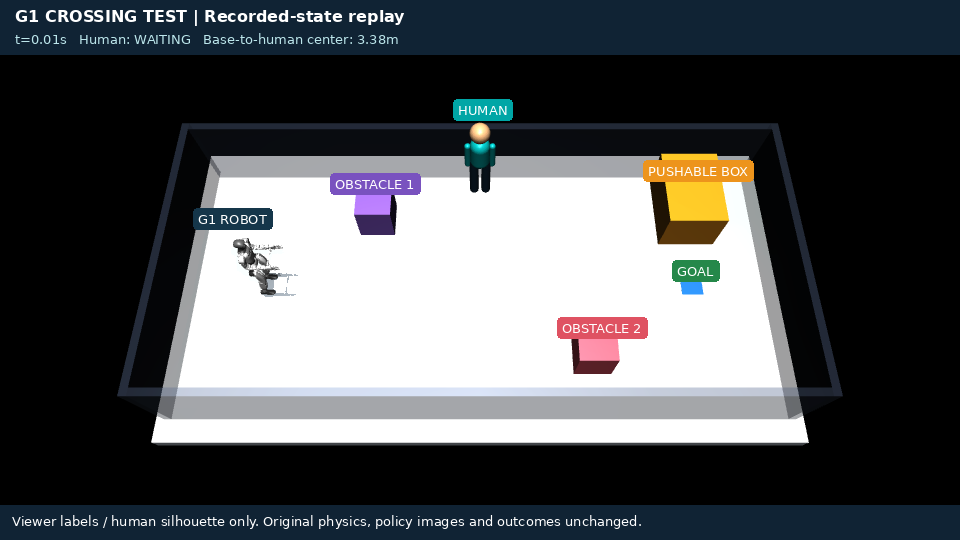
\includegraphics[width=\linewidth]{figures/humanoid_scene.png}
\caption{실험 2의 G1 휴머노이드 횡단 장면: 장애물 2개, 밀 수 있는 상자, 목표, 이동하는 사람.}\label{fig:env}
\end{figure}

\begin{table*}[!t]
\centering\small
\caption{두 실험의 조건}\label{tab:setup}
\begin{tabularx}{\textwidth}{@{}p{24mm}YY@{}}
\toprule
항목 & 실험 1: 로봇팔 pick-and-place & 실험 2: 휴머노이드 이동 \\
\midrule
시뮬레이터 & LIBERO-Spatial~\cite{libero} (robosuite~\cite{robosuite}·MuJoCo~\cite{mujoco}) & MuJoCo~\cite{mujoco} \\
로봇 & Franka Emika Panda 7자유도 + 평행 그리퍼~\cite{panda} & Unitree G1 29자유도~\cite{g1} \\
정책·제어 & GR00T~N1.7 공개 체크포인트(VLA)~\cite{groot,grootrepo}, 1회 추론당 8단계 동작 & 상위 LLM Agent(GPT-6 Luna) + 경로 계획·추종 + GR00T 보행 정책~\cite{wbc} \\
작업 & 테이블 중앙의 검은 그릇을 집어 접시에 놓기 & 상자·장애물·횡단하는 사람이 있는 통로에서 목표 도달 \\
성공 판정 & LIBERO 기본 판정(그릇이 접시 위), 약 15초(300 \gl{step}{제어 단계}) 이내 & 목표 반경 0.25\,m 안 1초 이상 체류, 로봇 판단 20회 이내 \\
시도 횟수 & 3세트(시드 661·673·677) $\times$ 2회 = 방법당 6회, 세트별 공통 시작 장면 2회는 평가 전 실행으로 제외 & 3세트 $\times$ 6회 = 방법당 18회, 세트별 공통 시작 장면 1회는 평가 전 실행으로 제외 (예비 실험: 1세트, 방법당 유효 4회) \\
공통 시작 장면 & 세트별 처음 2회, 두 방법이 같은 무작위 장면 사용 & 세트별 처음 1회, 두 방법이 같은 기본 장면 사용 \\
변경 규칙 & 10개 변수 자유 선택 & 시작 장면에서 변수 1개·2개 변경 교대, 최소 변경량은 변수 범위의 10\% \\
탐색 LLM & GPT-6 Luna Pro, 시도마다 제안 1건, 응답 제한 300초 & GPT-6 Luna, 시도마다 제안 1건 \\
측정 & 접촉 시간·접촉력, 그릇 이동·낙하, 그릇–접시 거리 & 로봇 기능(경로 계획, 상자 밀기) 실행 결과, 목표 거리, 자세, 사람과의 거리 \\
\bottomrule
\end{tabularx}
\end{table*}

\begin{table}[!t]
\centering\footnotesize\setlength{\tabcolsep}{3pt}
\caption{장면 변수와 범위}\label{tab:axes}
\begin{tabularx}{\linewidth}{@{}p{23mm}cY@{}}
\toprule
환경 요소 & 변수 수 & 범위 \\
\midrule
\multicolumn{3}{@{}l}{\textit{실험 1: 로봇팔 (테이블 좌표, m·rad)}} \\
그릇 X / Y & 2 & $[-0.10,-0.05]$ / $[-0.01,0.01]$ \\
접시 X / Y & 2 & $[0.06,0.10]$ / $[0.19,0.24]$ \\
장애물 X / Y & 2 & $[-0.24,-0.0075]$ / $[0.09,0.12]$ \\
장애물 폭·깊이·높이 & 3 & 폭·깊이 $[0.02,0.06]$, 높이 $[0.02,0.17]$ \\
장애물 회전 & 1 & $[-\pi/2,\pi/2]$ \\
\midrule
\multicolumn{3}{@{}l}{\textit{실험 2: 휴머노이드}} \\
물체·바닥 물성 & 3 & 상자 질량 0.2--10\,kg, 마찰계수 0.05--1.5 \\
통로·상자 배치 & 2 & 통로 폭 1.6--4.0\,m, 상자의 가로 위치(통로 가장자리--중앙) \\
장애물 2개 & 12 & 각각 위치·크기·높이·회전 \\
목표 부근 상자 & 1 & 진행 방향 위치 6.8--7.5\,m \\
사람 이동 & 3 & 위치 3.65--4.35\,m, 속도 0.1--1.5\,m/s, 출발 거리 0.5--5\,m \\
\bottomrule
\end{tabularx}
\end{table}

그림~\ref{fig:env}는 실험 2의 장면이고, 표~\ref{tab:setup}과 표~\ref{tab:axes}는 두 실험의 조건과 환경 변경 범위다. 
두 실험 모두 AFS와 Random 테스트는 같은 로봇, 작업, 성공 판정, 환경 변경 범위, 시도 횟수를 사용한다.
실험은 random seed로 구분한 \gl{set}{독립 실험 세트}(이하 세트) 단위로 반복하였다. 
각 세트의 처음 실행은 두 방법이 같은 장면을 쓰는 \gl{stage}{공통 시작 장면}이고, 그 이후 각 방법이 스스로 고른 시험을 \gl{stage}{탐색 단계}라 한다.
AFS는 같은 세트 안의 자기 실행 이력만 참고하며, 다른 방법이나 과거 실험의 결과를 가져오지 않는다.
로봇팔 실험에서 작업과 무관한 나머지 물체 배치는 모든 실행에서 같고, 방해용 검은 그릇 1개는 작업 영역 밖에 고정하였다.
휴머노이드 실험에서 판정 불가로 제외된 실행도 시도 횟수에 포함되며, 제외 후 재실행하지 않고 다음 순서로 진행한다.
휴머노이드 본 실험 3세트의 seed는 결과를 보기 전에 운영체제 random number로 정했으며(부록 A), 같은 세트를 AFS와 Random 테스트가 공유한다. 
앞서 수행한 예비 실험(1세트, GPT-6 Luna Pro, 로봇 판단 10회 이내)은 6절의 사례 분석에 사용한다.

본 과제는 SLAM~\cite{slam}, 물체 검출, 위치 추정 같은 인식 기술을 평가하지 않으므로, 휴머노이드 실험에서는 이 기술들로 얻어야 할 정보를 시뮬레이터의 실제 값으로 제공하도록 제약하였다. 
로봇의 LLM은 매 프레임이 아니라 판단할 때마다 그 시점의 카메라 영상 1장과 함께 로봇 자신과 장애물·상자·사람의 정확한 위치·크기·방향(사람은 별도 표시), 목표 위치, 직전 행동의 실행 결과를 받는다. 
이동 중에는 경로 계획·추종기가 같은 실제 위치·크기 정보로 경로를 갱신하지만, LLM은 응답을 생성하는 동안 새 정보를 받지 않아 판단 시점과 실행 시점의 사람 위치가 다를 수 있다.
따라서 실험 2의 결과는 인식 정보가 주어진 조건에서 계획·행동 단계의 실패를 탐색한 것이며, 사람을 보고 기다린 판단도 영상에서 나왔는지 위치 정보에서 나왔는지는 구분하지 않는다. 
실험 1의 VLA 정책은 카메라 영상과 관절 상태로 직접 동작하므로 인식이 정책 안에 포함된다.
